\documentclass[10pt]{article}
\usepackage[utf8]{inputenc}
\usepackage[T1]{fontenc}
\usepackage{amsmath}
\usepackage{amsfonts}
\usepackage{amssymb}
\usepackage[version=4]{mhchem}
\usepackage{stmaryrd}
\usepackage{hyperref}
\hypersetup{colorlinks=true, linkcolor=blue, filecolor=magenta, urlcolor=cyan,}
\urlstyle{same}
\usepackage{graphicx}
\usepackage[export]{adjustbox}
\graphicspath{ {./images/} }

\title{Influence of processing parameters on the evolution of melt pool, porosity, and microstructures in Ti-6Al-4V alloy parts fabricated by selective laser melting }


\author{J. J. S. Dilip ${ }^{1,2}$ - Shanshan Zhang ${ }^{1}$ - Chong Teng ${ }^{3}$ - Kai Zeng ${ }^{3}$ - Chris Robinson ${ }^{3}$ -\\
Deepankar Pal ${ }^{3} \cdot$ Brent Stucker $^{3}$}
\date{}


%New command to display footnote whose markers will always be hidden
\let\svthefootnote\thefootnote
\newcommand\blfootnotetext[1]{%
  \let\thefootnote\relax\footnote{#1}%
  \addtocounter{footnote}{-1}%
  \let\thefootnote\svthefootnote%
}

%Overriding the \footnotetext command to hide the marker if its value is `0`
\let\svfootnotetext\footnotetext
\renewcommand\footnotetext[2][?]{%
  \if\relax#1\relax%
    \ifnum\value{footnote}=0\blfootnotetext{#2}\else\svfootnotetext{#2}\fi%
  \else%
    \if?#1\ifnum\value{footnote}=0\blfootnotetext{#2}\else\svfootnotetext{#2}\fi%
    \else\svfootnotetext[#1]{#2}\fi%
  \fi
}

\begin{document}
\maketitle
Received: 13 December 2016/Accepted: 2 August 2017/Published online: 9 August 2017

(C) Springer International Publishing AG 2017

\begin{abstract}
Selective laser melting involves melting and solidification of metal powder particles in a track-by-track and layer-by-layer method to fabricate 3D parts. The present investigation focuses on understanding the effect of laser power and scan speed on the evolution of melt pool, porosity and multiple thermal cycling effects on the microstructure in parts fabricated using selective laser melting. In this study, Ti-6Al-4V pre-alloyed powder was used to produce single-track deposits and bulk parts. Using different combinations of laser power and scan speeds, single-track deposits and bulk parts were produced. The cross-sections of the single-track deposits and bulk samples were prepared for metallographic observations and the melt pool shape and size and porosity were evaluated. When a low energy density was applied the un-melted powder particles produced irregularly shaped porosity, and a high energy density resulted in rounded porosity, which was due to keyhole effects. The samples produced with a proper combination of power and speeds were fully dense. Further, microstructural development under the influence of process condition was highlighted. Overall, the study demonstrates a good correlation between the single-track melt pool geometries, porosity in bulk parts and also demonstrates the microstructural inhomogeneity during deposition.
\end{abstract}

\footnotetext{$\boxtimes$ J. J. S. Dilip

\href{mailto:samueldilip@gmail.com}{samueldilip@gmail.com}

1 Department of Industrial Engineering, Rapid Prototyping Center, University of Louisville, Louisville, KY 20292, USA

2 HP Labs, 1501 Page Mill Road, Palo Alto, CA 94304, USA

3 3DSIM, 1794 Olympic Parkway, Suite 110, Park City, UT 84098, USA
}Keywords Additive manufacturing $\cdot$ Selective laser melting $\cdot$ Ti-6Al-4V alloy $\cdot$ Single-track deposits

\section*{1 Introduction}
Additive manufacturing belongs to the group of manufacturing technologies where 3D parts are fabricated by material addition in a layer-by-layer fashion, usually from a computer-aided design model [1]. Additive manufacturing technologies offer enhanced design capabilities for geometric freedom that allows producing parts which are otherwise not possible to fabricate with traditional manufacturing processes. There are various additive manufacturing processes such as selective laser melting, direct laser deposition, electron beam melting, wire-feed additive manufacturing, shape deposition modeling, ultrasonic consolidation, binder jetting, and friction freeform fabrication for producing metallic components [1-8]. Titanium alloys are used in several structural applications due to their lower density, high strength to weight ratio, corrosion resistance, and elevated temperature properties [9]. Traditionally, titanium alloys are made by vacuum induction re-melting and carefully controlled thermo-mechanical processing to tune the microstructure that will demonstrate satisfactory mechanical properties. Although manufacturing methods are well established for titanium alloys, the high production cost limits the use of these alloys. Additive manufacturing could provide a means to fabricate parts in titanium alloys at a lower cost. Among the various grades of titanium alloys, Ti-6Al-4V $(\alpha+\beta$ alloy) is the most popular and finds its applications in aerospace, automotive, biomedical, defence and industrial sectors $[9,10]$. The alloy has good weldability characteristics, making it amenable for SLM.

Of the commercially available additive manufacturing technologies, selective laser melting (SLM) is one of the most popular and successful powder-bed fusion based additive manufacturing processes. In SLM, consolidation of metal powder is achieved by melting and solidifying a small volume of material in a track-by-track and layer-bylayer fashion using a high-intensity laser. In other words, the laser beam scans over a layer of powder in a straight line and melts the powder particles under the beam and creates a small molten pool of metal. As the laser beam traverses, it leaves a thin track of solidified metal behind. On repeating the single track deposit with a well-defined overlap (hatch spacing), a layer of cross-section is produced. Upon repeating this layer-by-layer deposition, an entire part is constructed [1]. A simple schematic of the SLM process showing track-by-track and layer-by-layer deposition is presented in Fig. 1 [11]. SLM is controlled by various processing parameters such as laser power $(P)$, scanning speed $(v)$, layer thickness $(t)$ and hatch spacing (h). These parameters define energy density of the process as [12]:

$E=\frac{P}{v \times h \times t}$.

Although energy density is a measure of the energy input to the process, there are other factors such as the composition of the metal, atmosphere used, scan pattern, and powder-bed temperature, which also play a significant role [13]. All the parameters mentioned above mutually influence each other, but the degree of effect by each parameter is not well understood. Therefore, studying the basic element of SLM, i.e., the single-track deposits, will provide a deeper understanding of the process and could assist in identifying a process window for optimizing parameters, particularly when dealing with new alloy systems [11].

In recent times, a great deal of work has been carried out on the Ti-6Al-4V alloy for optimization of parameters, microstructural characterization, and mechanical property evaluation using SLM [12-15]. Gong et al. [11] reported a strategic method to arrive at optimum parameters through producing single beads on the base plate and extended their work to characterize a test pad $(10 \mathrm{~mm} \times 10 \mathrm{~mm} \times 1 \mathrm{~mm})$ with multiple layers. Gong et al. described the effect of power and scan speed on the melt pool geometry, and also showed surface topology of multi-layer pads, which were evaluated for porosity and quality evaluation. However, a detailed study on porosity and microstructures was not reported. Also, in their study, the single-track deposits were made on a base plate made on a Ti plate. Very recently, Yang et al. [16] investigated the role of melt pool on microstructure and mechanical properties of Ti-Al-4V. The study explores the use of a keyhole mode over a conduction mode for SLM deposits, and it was noticed that the conduction mode provided denser parts with better mechanical properties. In their experiments, the single-track deposits were made on a pure Ti plate. In both the case studies, single-track deposits resulted in a significant amount of dilution with the base plate alloy. It is well known that dilution contributes to a change in the local composition of the melt pool, thus changing the melting temperature of the Ti-6Al-4V alloy powder in the local single-track vicinity. In other words, the volume of the melt pool created will be different from the actual volume when the melting temperature is changed. Hence, the estimate of melt pool size will probably be close to the actual one but not a true representation of the melt pool size. Therefore, a study on single tracks made of the same alloy (Ti-6Al-4V plate) is necessary to have an accurate measure of melt pool geometry. Thijis et al. [15] studied the influence of process parameters on porosity and the development of microstructures. In their study, they varied the energy density of the process (by altering the scan speed and hatch spacing) and presented its effects on porosity. They described the evolution of grain (elongated) structure in the deposits due to epitaxial growth, and the fast cooling in SLM resulting in a fully martensitic phase. The martensite phase formed will experience multiple thermal cycling effects during track-by-track and layer-by-layer material deposition and therefore, finally result in a microstructure containing a hierarchical structure of martensite [17].

The quality and the properties of parts produced by SLM primarily rely on the nature of single-track deposits, overlap between the layers, and thermal history. It is\\
Fig. 1 A schematic the SLM process showing track-by-track and layer-by-layer deposition of material [9]

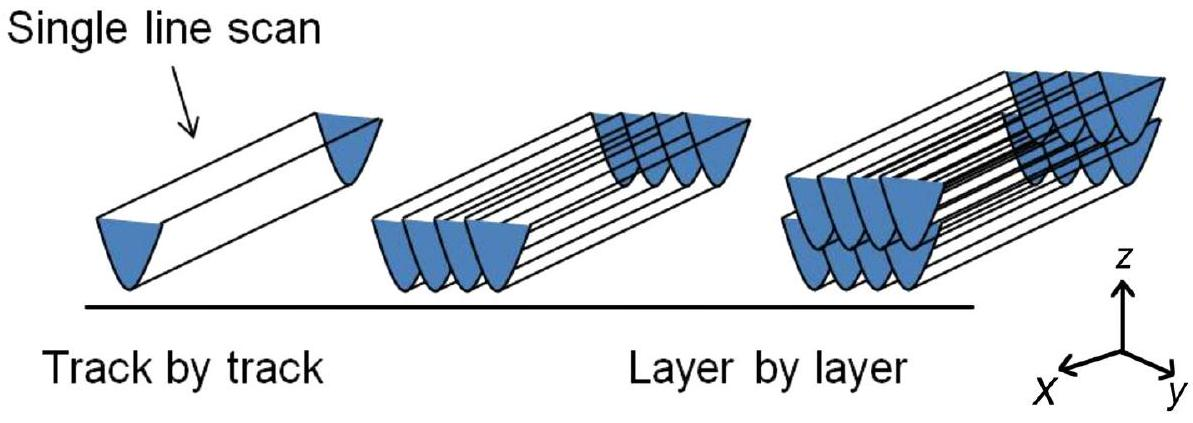
\includegraphics[max width=\textwidth, center]{2024_02_28_5b6806184856c64a957ag-02}\\
essential to study and understand the mechanism of formation of single-track deposits based upon processing parameters such as scanning speed, laser power, and powder layer thickness. In the present work, we attempt to produce single-track deposits on Ti-6Al-4V alloy plate. The objectives of the present work are (i) to study the influence of process parameters on single-track deposits on the evolution of the melt pool and (ii) to understand the effect of process parameters on porosity and microstructures in bulk parts. We believe that this work will provide further insights into understanding the SLM process and could assist in developing a process window for faster identification of optimum process parameters.

\section*{2 Experimental work}
Ti-6Al-4V pre-alloyed powder $(15-45 \mu \mathrm{m})$ supplied by LPW Technology Inc., Pittsburg, PA, USA, was used in the present study. The powder was characterized using SEM for examining the particle size, shape and distribution. An EOS M270 direct metal laser sintering (DMLS) system with $\mathrm{Yb}$-fiber laser (nominal maximum power $200 \mathrm{~W}$ ) was used to fabricate the single-track deposits and bulk sample parts. Experiments were performed with multiple combinations of laser power and scan speeds to produce singletrack deposits and bulk samples (Table 1). A layer thickness of $30 \mu \mathrm{m}$ was maintained for all the test samples.

When a thin wall equivalent to the beam diameter is made, the laser will scan as one single line, and thus make a single line of deposit. It is known that support structures in an EOS system have a minimum smallest dimension of $100 \mu \mathrm{m}$ [18]. Therefore, single-track deposits can be produced utilizing line support structure settings. To achieve a single line deposit, thin wall sections with the dimension of $0.1 \mathrm{~mm} \times 0.1 \mathrm{~mm} \times 100 \mathrm{~mm}$ were made using Materialise Magics software and placed at a height of $5 \mathrm{~mm}$. Then support structures were generated under these thin wall sections/parts. It is to be noted that these thin walls are sacrificial parts and will be deleted once supports are generated. Then parameters (listed in Table 1) with various laser powers and scan speeds were applied to each of the single line supports. A Ti-6Al-4V alloy plate of $3.3 \mathrm{~mm}$ was placed on the build platform, and then a layer of $30 \mu \mathrm{m}$ thick powder was spread. A single exposure laser scan was applied to scan one single layer. In this method, single-

Table 1 Single-track deposits and bulk samples made with various powers and scan speeds

Laser power (W)

$50,100,150,195$

Scan speed $(\mathrm{mm} / \mathrm{s})$

$500,750,1000,1200$

\begin{center}
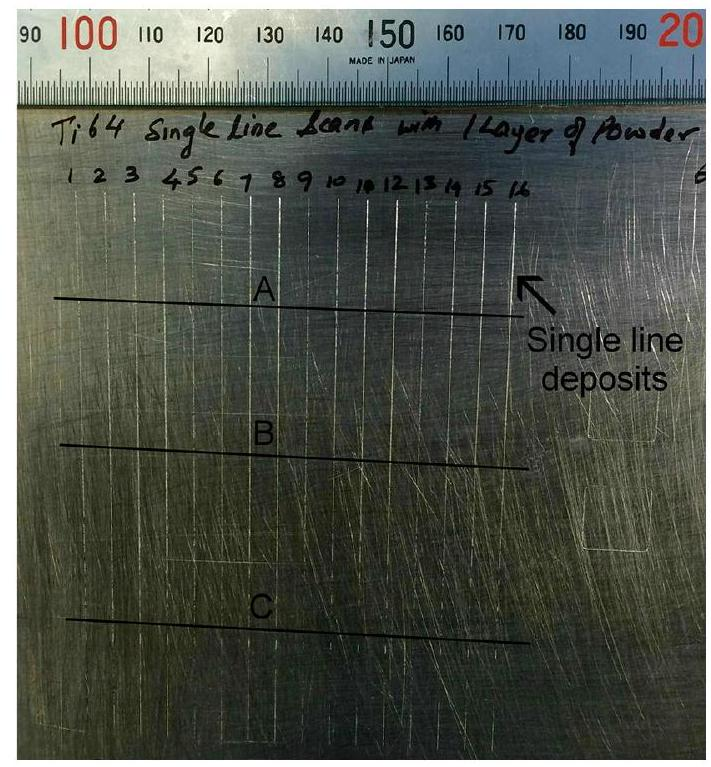
\includegraphics[max width=\textwidth]{2024_02_28_5b6806184856c64a957ag-03}
\end{center}

Fig. 2 Photograph of the Ti-6Al-4V plate showing single-track deposits (note: single tracks appear as thin vertical lines)

track deposits on a Ti-6Al-4V alloy plate (thickness $3.3 \mathrm{~mm}$ ) were made. The single-track deposits were pre-set at $5 \mathrm{~mm}$ distance apart. Single-track deposits of a length of $100 \mathrm{~mm}$ were made on the Ti-6Al-4V plate. A photograph of the plate containing the single-track deposits is shown in Fig. 2. The single-track deposits were cut at $1 / 3,1 / 2$ and $2 / 3$ lengths (sections A, B, and C) for microscopy studies. The top surface of the single line deposit was examined under a scanning electron microscope. Later, bulk samples $(10 \mathrm{~mm} \times 10 \mathrm{~mm} \times 5 \mathrm{~mm})$ were built using the same set of parameters. The bulk samples were sectioned, polished, and etched with Keller's reagent. The bulk samples were characterized using optical microscopy for examining the porosity and microstructures. The amount of porosity in the samples was estimated as per ASTM E-562.

\section*{3 Results and discussion}
Ti-6Al-4V pre-alloyed powder was characterized using SEM. Figure 3a shows morphology and distribution of the powder particles. Particle size and distribution were determined by measuring the diameters of individual particles from several different micrographs. The particles have a particle size distribution between 15 and $45 \mu \mathrm{m}$. The powders showed spherical morphology with bi-modal size distribution. Figure $3 b$ shows a SEM micrograph revealing characteristic micro-dendritic features on the surface of powder particles. This phenomenon occurs due to nucleation and growth of dendrites in the powder particle during slow cooling occurring in atomization process [8].

Fig. 3 a A low magnification SEM micrograph of Ti-6Al-4V powder. b A high magnification SEM micrograph of powder particles\\
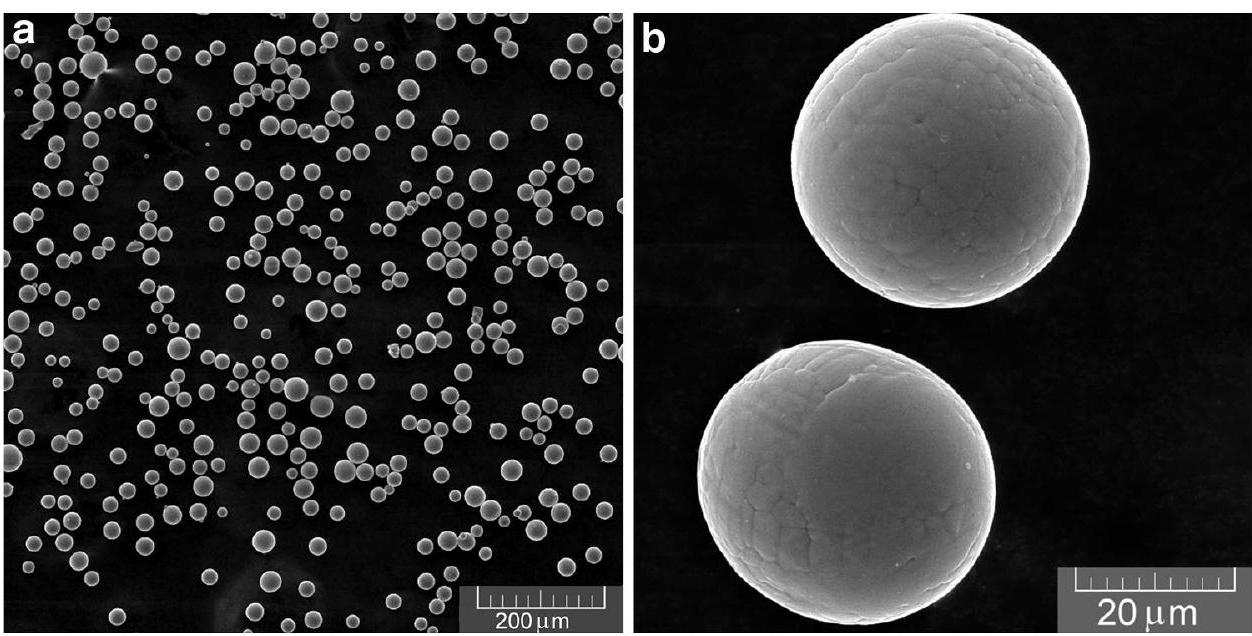
\includegraphics[max width=\textwidth, center]{2024_02_28_5b6806184856c64a957ag-04(1)}\\
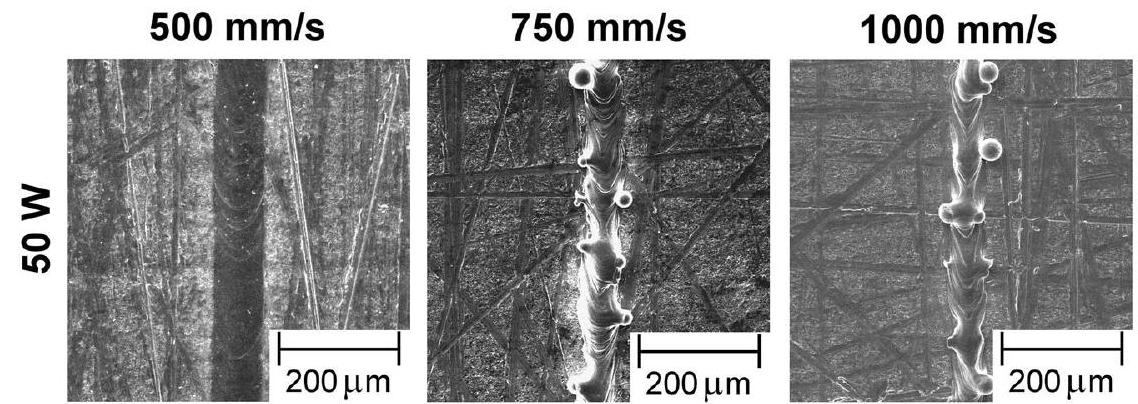
\includegraphics[max width=\textwidth, center]{2024_02_28_5b6806184856c64a957ag-04}

$1200 \mathrm{~mm} / \mathrm{s}$\\
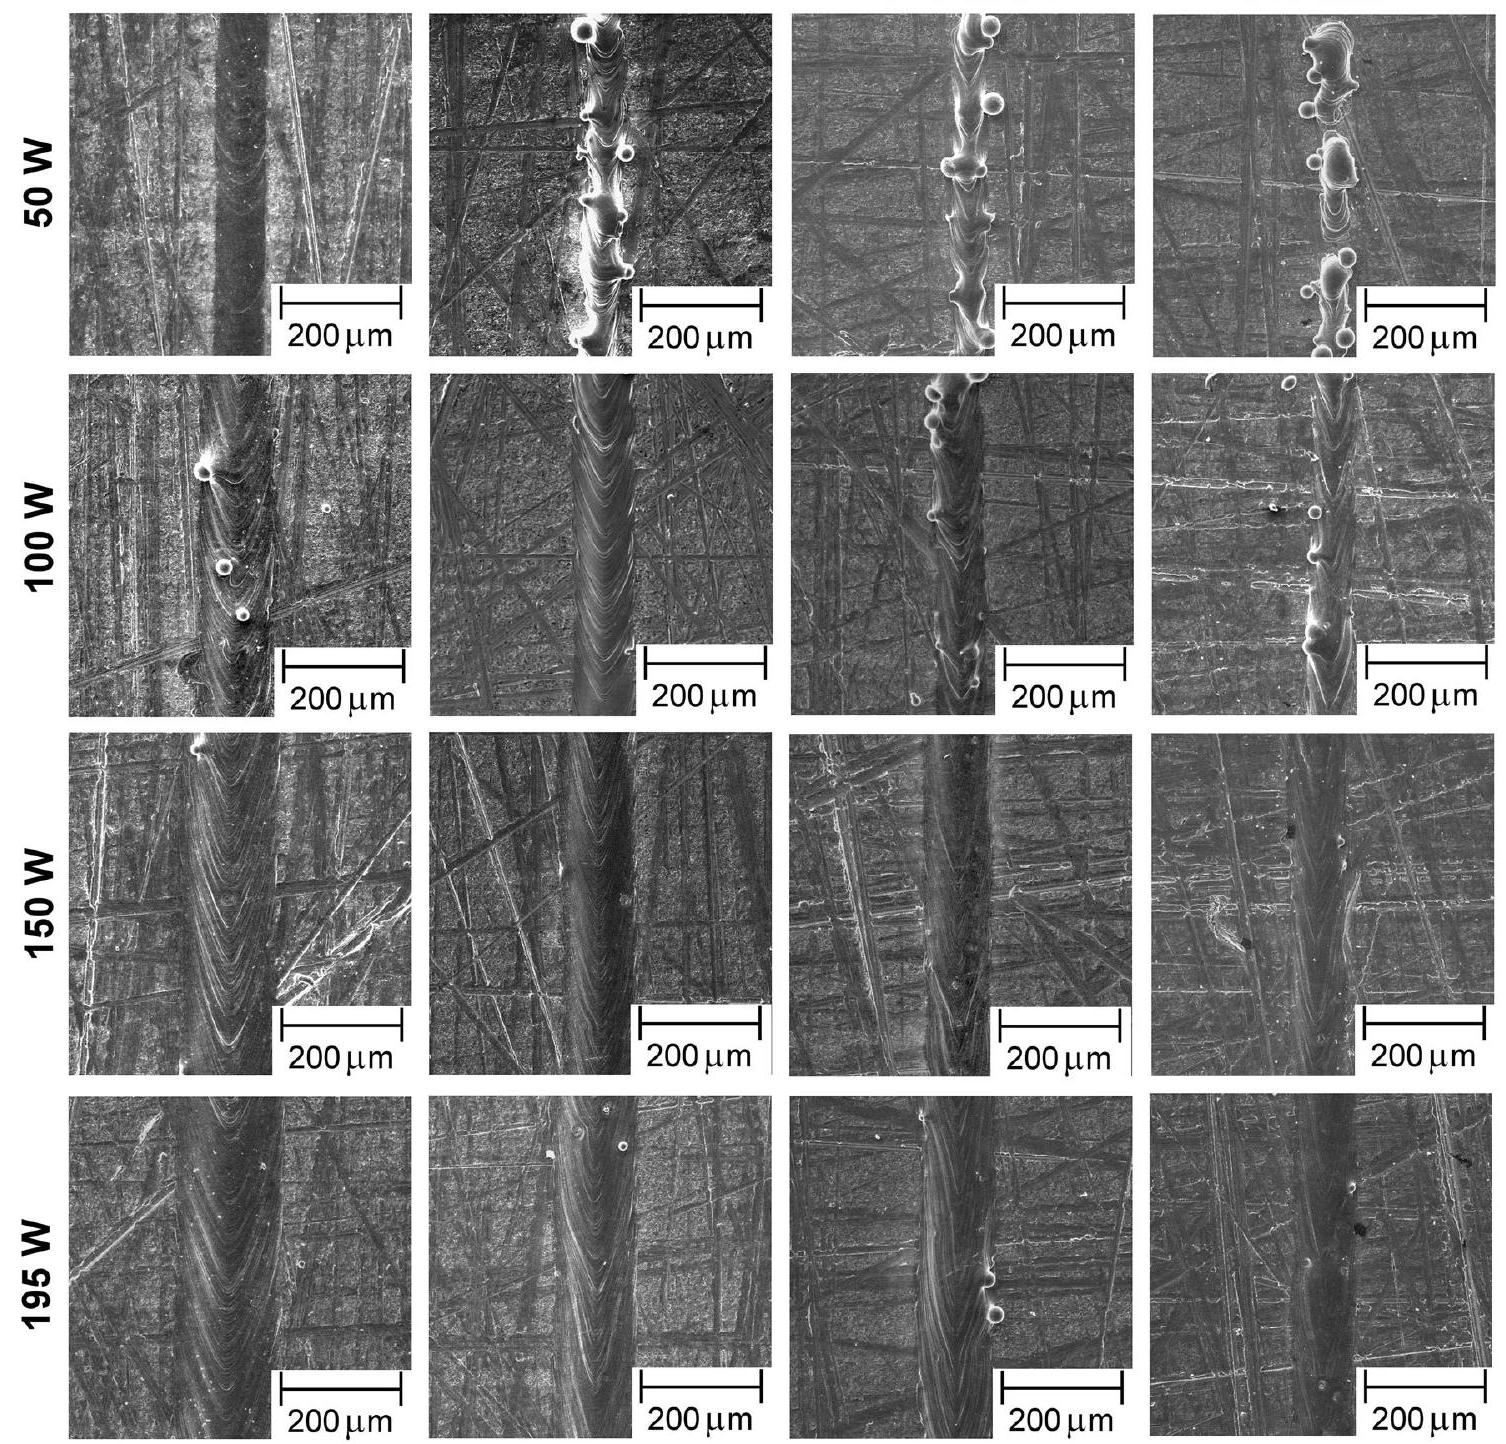
\includegraphics[max width=\textwidth, center]{2024_02_28_5b6806184856c64a957ag-04(2)}

Fig. 4 SEM images showing the top surface morphology of the single-track deposits

The top surface of the single line deposits was observed under SEM, and the results are presented in Fig. 4. The single-track deposit scanned with low laser power, and slow scan speed ( $50 \mathrm{~W}$ and $500 \mathrm{~mm} / \mathrm{s}$ ) shows a continuous, and a uniform weld bead. Keeping the laser power constant $(50 \mathrm{~W})$, with an increase in the scan speed the single-track deposit was noticed to become inconsistent and discontinuous $(1000 \mathrm{~mm} / \mathrm{s})$, and eventually resulting in fragmentation of tracks $(1200 \mathrm{~mm} / \mathrm{s})$, commonly referred to as balling [11]. Balling appears spherical in shape (as shown in Fig. 5, $50 \mathrm{~W}, 1200 \mathrm{~mm} / \mathrm{s}$ ) and bulging upwards which is a result of the dominant surface tension forces of the molten alloy. When such a sets of parameters are applied to fabricate the bulk parts, they may result in a significant amount of porosity $[9,11]$. Keeping scan speed constant, and with an increase in the laser power, the single bead deposit shows an increase in width. This increase in the width is due to the higher intensity of the laser beam, which causes a higher volume of melting and results in a wider and deeper melt pool [11] (Fig. 6). In the case of single tracks deposited with a laser power of 100,150 , and $195 \mathrm{~W}$, the bead width was observed to decrease with an increase in scan speed; however, balling phenomenon was not observed at these higher laser power settings.

The single-track deposits produced on a Ti-6Al-4V alloy plate were sectioned and prepared for microstructural\\
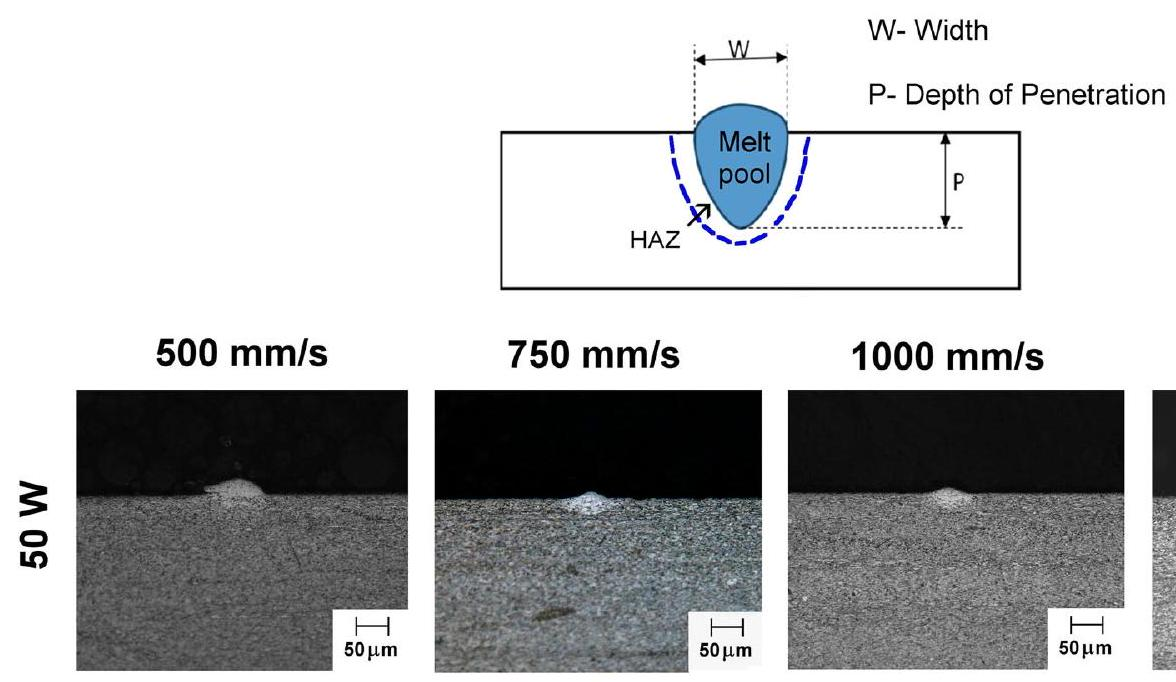
\includegraphics[max width=\textwidth, center]{2024_02_28_5b6806184856c64a957ag-05}

\section*{$1200 \mathrm{~mm} / \mathrm{s}$}
\begin{center}
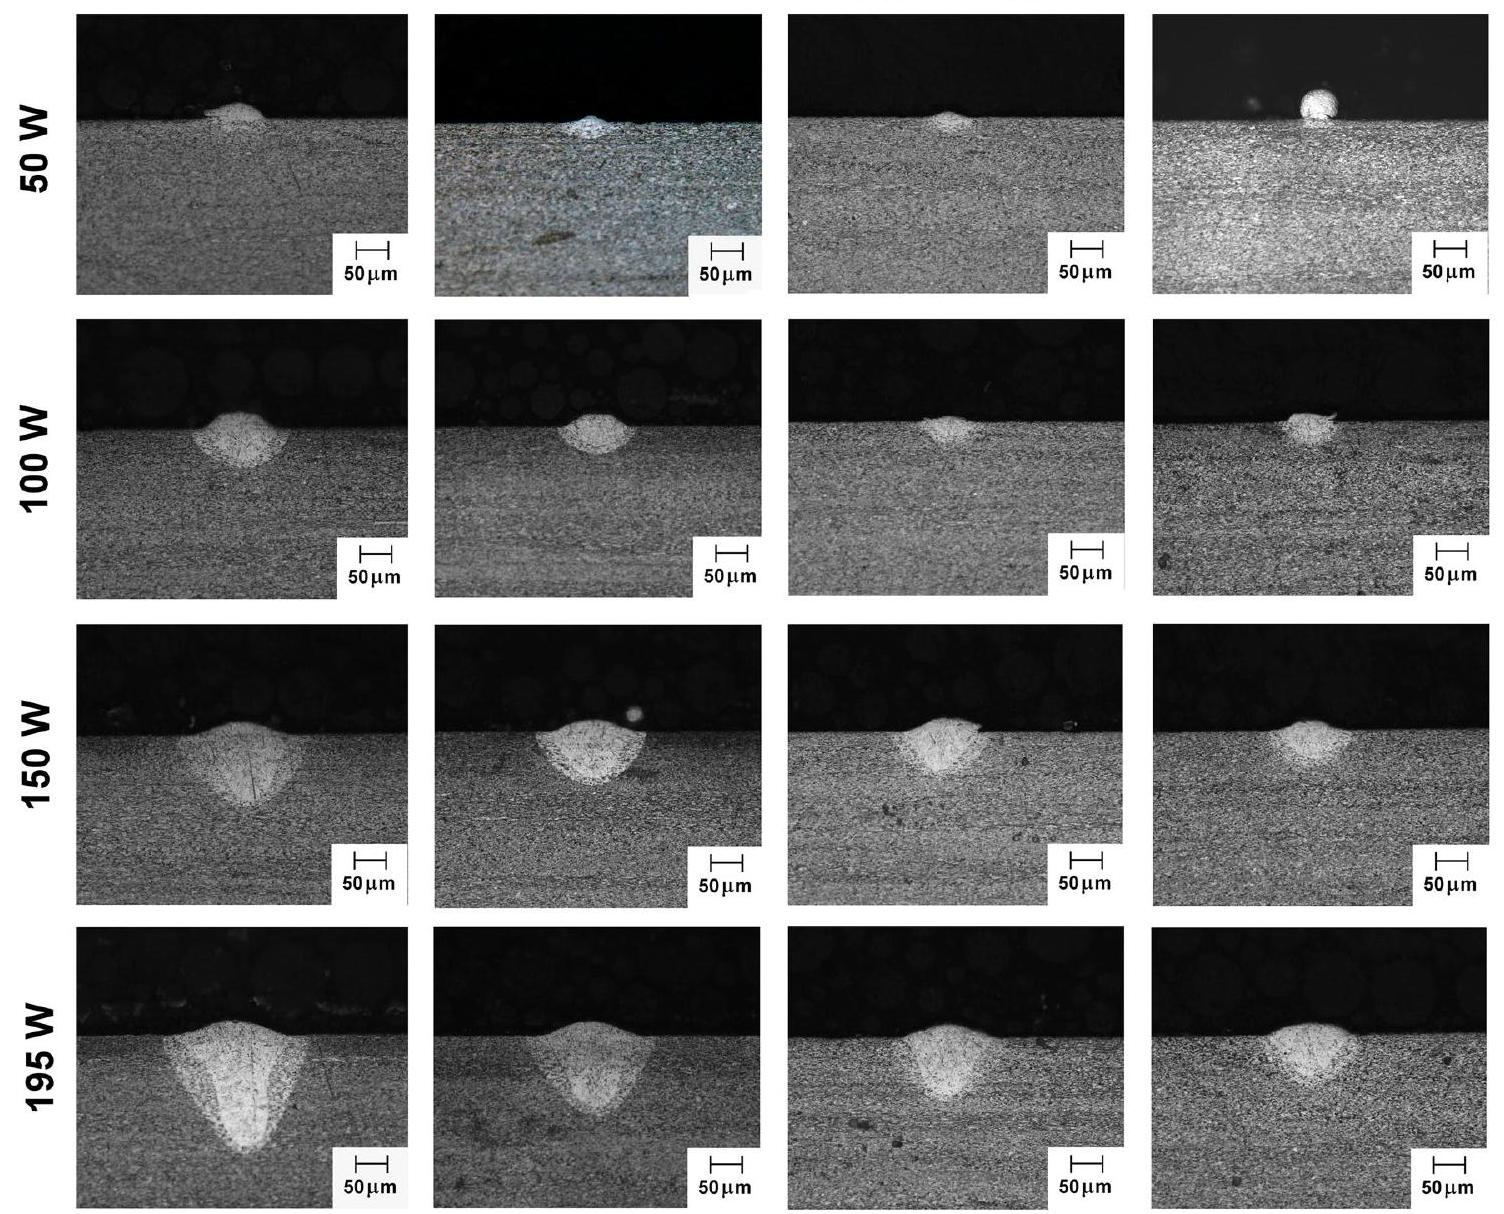
\includegraphics[max width=\textwidth]{2024_02_28_5b6806184856c64a957ag-05(1)}
\end{center}

Fig. 5 Cross-section optical micrographs of the single-track deposits produced on a Ti-6Al-4V alloy plate using various parameter combinations\\
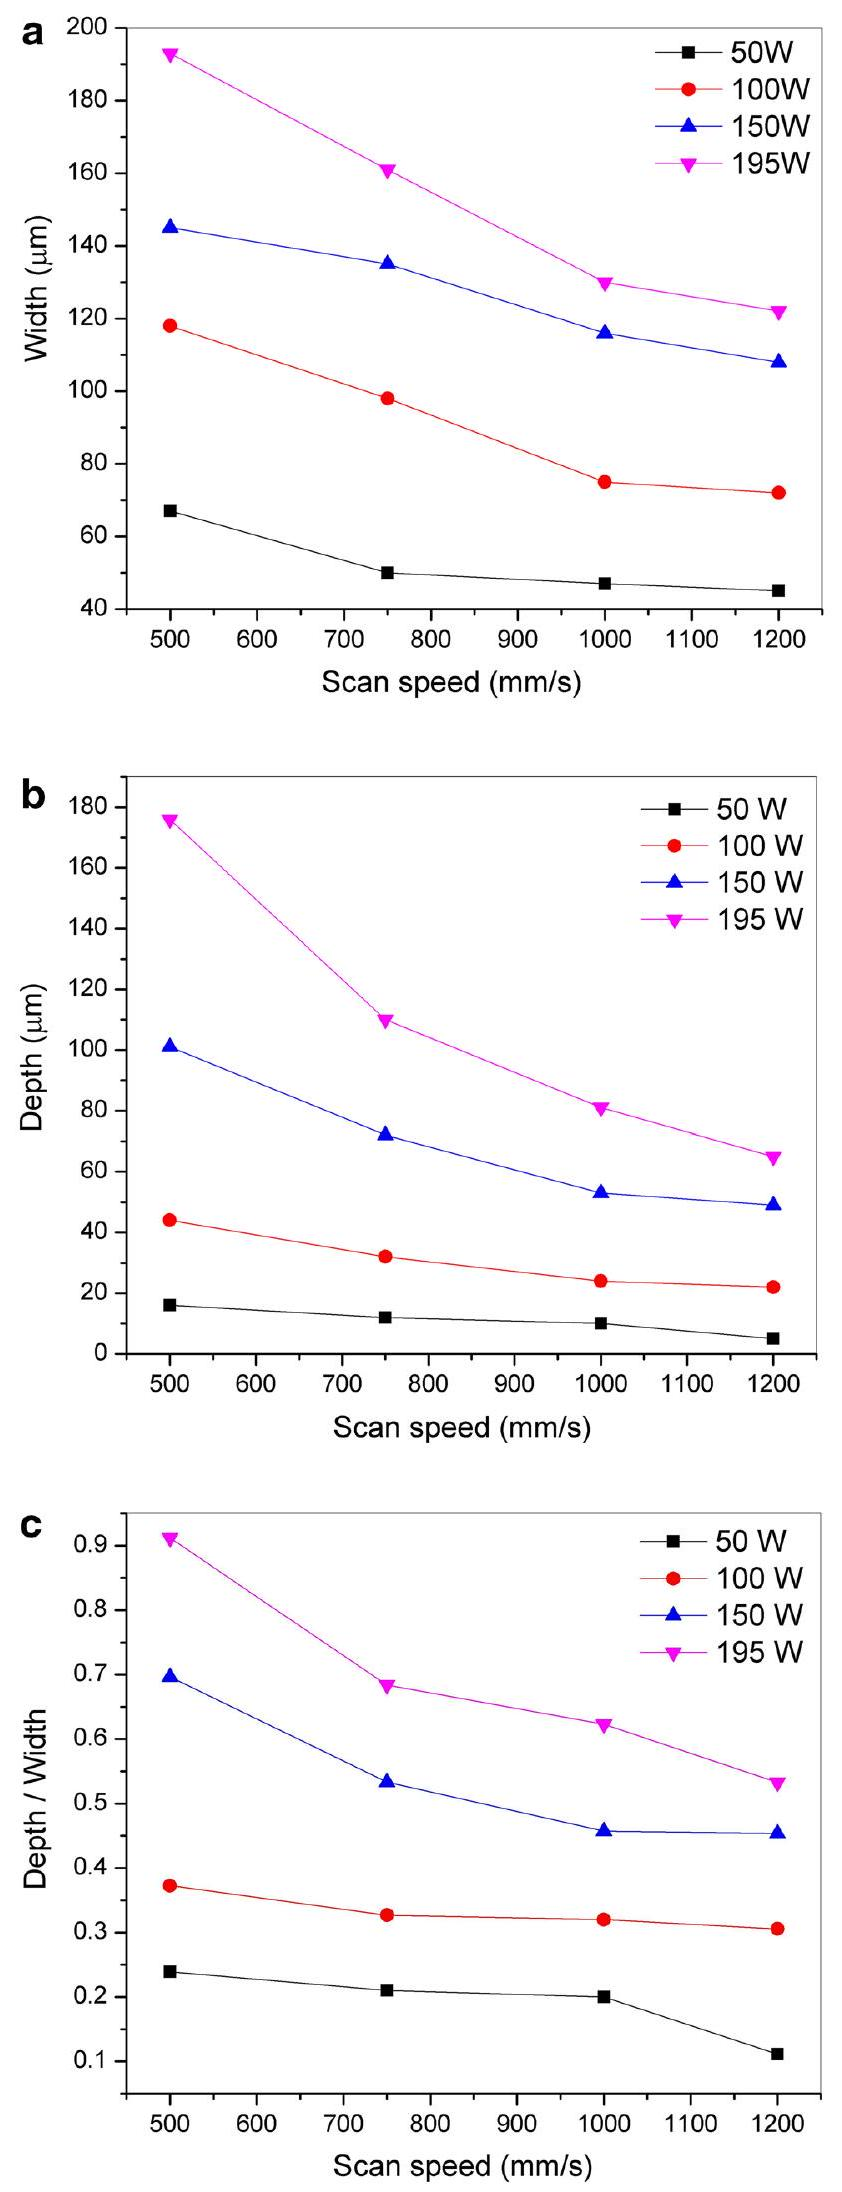
\includegraphics[max width=\textwidth, center]{2024_02_28_5b6806184856c64a957ag-06}

Fig. 6 Variation of melt pool geometry on process parameters a bead width, $\mathbf{b}$ depth of penetration and $\mathbf{c}$ depth-to-width ratio observations. The etched cross-sections were examined under an optical microscope, and the micrographs are presented in Fig. 5. The morphology, width, and depth of the single-track deposits can be clearly observed from the optical micrographs. At a power level of $50 \mathrm{~W}$ and scan speed of $500 \mathrm{~mm} / \mathrm{s}$, the energy was sufficient to melt the powder and a small portion of the base plate $(10 \mu \mathrm{m})$. When the scan speed was increased, the depth of the melted region was observed to decrease and eventually resulted in balling, which can be observed for the single track made with $50 \mathrm{~W}, 1200 \mathrm{~mm} / \mathrm{s}$. This phenomenon occurs due to the reduction in the energy density as the scan speed was increased according to Eq. 1 [10]. The melt pool depth was observed to increase significantly at lower scan speeds $(500 \mathrm{~mm} / \mathrm{s})$ and higher power levels particularly from $100 \mathrm{~W}$ (depth: $45 \mu \mathrm{m}$ ) to $195 \mathrm{~W}$ (depth: $176 \mu \mathrm{m}$ ). The melt pool geometry was observed to have a keyhole shape for the laser power of $195 \mathrm{~W}$, whereas for $100 \mathrm{~W}$ it was bowl shape. This remarkable change in melt pool shape with laser irradiation can be attributed to keyhole versus conduction modes of melting. For lower laser power, melting occurs by locally melting the alloy with heat transfer by conduction and convection inside the melt pool. In the later case, with a laser power of $195 \mathrm{~W}$, melting of the alloy occurs by keyhole mode, giving rise to deeper penetration. Keyhole is always associated with vaporization of the alloy and in many cases results in entrapped pores in the melt pool [16]. The single tracks with the parameter combinations of: $100 \mathrm{~W}-500 \mathrm{~mm} / \mathrm{s}$, $150 \mathrm{~W}-500 \mathrm{~mm} / \mathrm{s}, 150 \mathrm{~W}-750 \mathrm{~mm} / \mathrm{s}, 150 \mathrm{~W}-$ $1000 \mathrm{~mm} / \mathrm{s}, 195 \mathrm{~W}-1000 \mathrm{~mm} / \mathrm{s}$, and $195 \mathrm{~W}-1200 \mathrm{~mm} / \mathrm{s}$, have moderate energy input and provide consistent melt pool shape with sufficient depth of penetration (two to three layers deep). These parameters above when used with a well-defined melt pool overlap could provide a window of optimum processing conditions to produce fully dense parts. It is worth noting that the heat affected zone size close to the melt pool also varies with the energy density applied.

The overall effect of process parameters on the width and depth of the single-track deposits is presented in Fig. 6. Laser power and scan speed have a significant effect on the single-track melt pool geometry. The results in Fig. 6a indicate for all power levels, an increase in scan speed shows a decrease in bead width. An increase in laser power results in an increase in the width, due to the increase in the energy density. The effect of process parameters on the depth of penetration can be observed from Fig. 6b. The results indicate that both laser power and scan speed significantly affect the amount of melting and the depth penetration. When the energy density is high (high power -low speed), the result shows a higher depth of penetration and melting up to $175 \mu \mathrm{m}$ (equivalent to six layers melted\\
beneath). The effect of process parameters on the depth-towidth ratio is presented in Fig. 6c. For depth-to-width ratios around 0.37 to 0.6 , it has at least $2-3$ layers melted below and can ensure proper welding with the substrate. SLM can be considered very similar to laser welding, with high power levels and slow scan speeds, and a conduction mode similar to welding/deposition occurs, resulting in a deeper melt pool $[11,16,19,20]$.

Bulk sample parts of dimensions $10 \mathrm{~mm} \quad \times$ $10 \mathrm{~mm} \times 5 \mathrm{~mm}$ were fabricated using the parameters listed in Table 1. The SLM-built sample parts were cut and prepared for microstructural studies. The polished and etched cross-section surfaces of the as-built bulk samples are presented in Fig. 7. The effect of process parameters on the porosity/density of the sample can be clearly observed in Fig. 7. The samples made with parameters $50 \mathrm{~W}$ laser power and different scan speeds reveal irregular shape pores (dark) with sharp edges and also some unmelted powder particles in the micrographs. The porosity was observed to increase as the scan speed was increased. These results have a good match with the single-track melt pool observations. The sample with $100 \mathrm{~W}$ laser power and $500 \mathrm{~mm} / \mathrm{s}$ scan speed resulted in full density, and as the scan speed was increased the porosity in the parts showed a rise due to insufficient melting of the powder. With the higher laser power levels, 150 and $195 \mathrm{~W}$, a scan speed of $500 \mathrm{~mm} / \mathrm{s}$ showed round voids. The sample with $195 \mathrm{~W}$ laser power showed larger pore sizes in the cross-section. The formation of porosity in the deposits could be derived from the keyhole-shaped melt pool that developed while high power parameters were used. High energy density causes the alloy to melt and vaporize in some local regions; since the process is dynamic and quick, the vapors cannot escape fully and become entrapped in the melt pool, resulting in pores (which appear round) in the deposit [16, 19-22]. However, the pores when formed towards the top of the melt pool are not detrimental because re-melting causes gas to escape out of that layer during subsequent\\
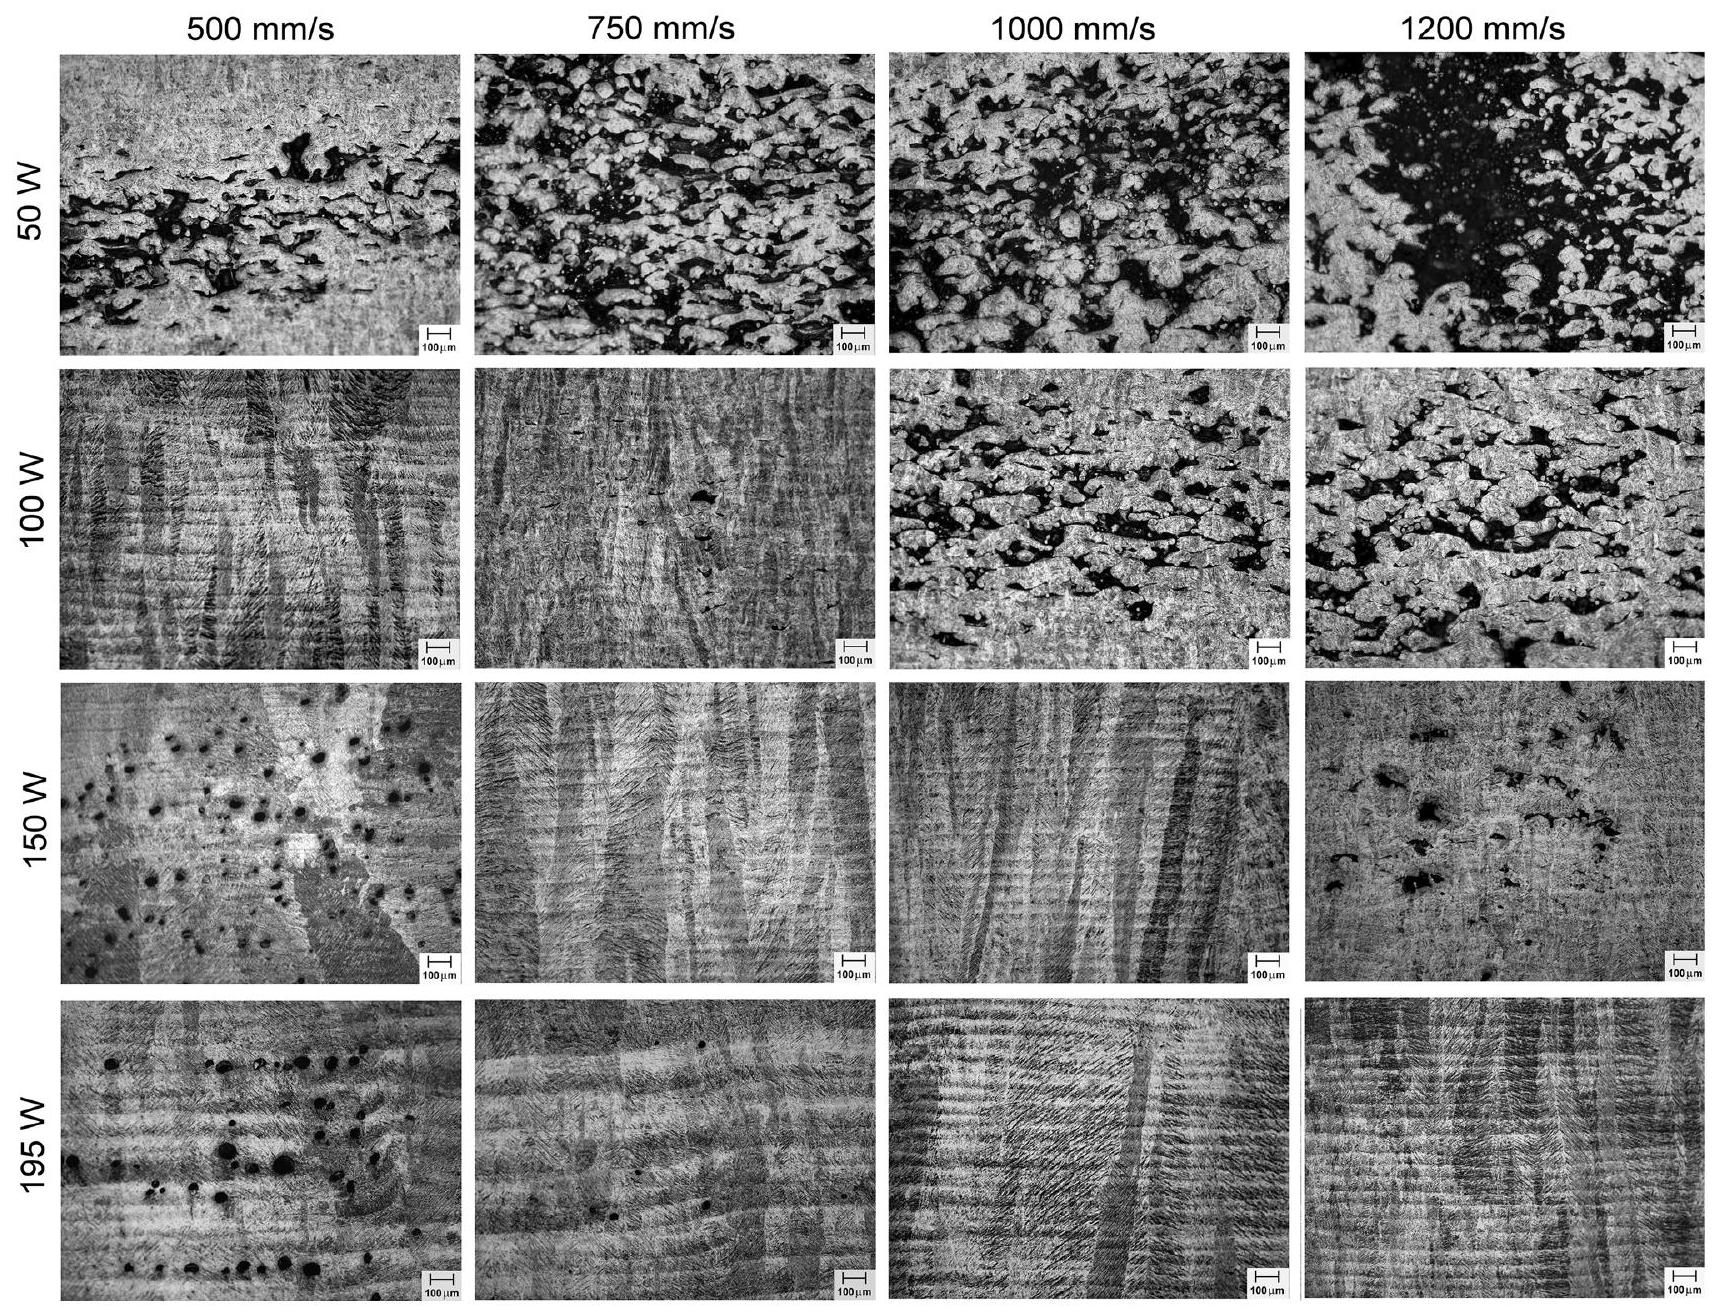
\includegraphics[max width=\textwidth, center]{2024_02_28_5b6806184856c64a957ag-07}

Fig. 7 Cross-section optical micrographs of the bulk samples showing variation in porosity based upon process parameters

Table 2 Calculated energy densities $\left(\mathrm{J} / \mathrm{mm}^{3}\right)$ for various parameters applied for producing bulk samples

\begin{center}
\begin{tabular}{lcccc}
\hline
Laser power $(\mathrm{W})$ & \multicolumn{2}{l}{Scan speed $(\mathrm{mm} / \mathrm{s})$} &  & 1200 \\
\cline { 2 - 5 }
 & 500 & 750 & 1000 & 13 \\
\hline
50 & 33 & 22 & 33 & 27 \\
100 & 66 & 44 & 50 & 41 \\
150 & 100 & 66 & 65 & 54 \\
195 & 130 & 86 & 33 &  \\
\hline
\end{tabular}
\end{center}

layer deposition. The pores formed deep inside, and in the lower end of the melt pool, are more detrimental $[9,11,15,19,22]$. Therefore, higher power and lower speed should be avoided for overcoming such adverse defects. The samples made with parameters: (i) $150 \mathrm{~W}$ and scan speeds 750 and $1000 \mathrm{~mm} / \mathrm{s}$, and (ii) $195 \mathrm{~W}$ and scan speeds 1000 and $1200 \mathrm{~mm} / \mathrm{s}$ were fully dense.

The energy density gives an estimate of the energy input to the SLM process. Energy density estimation applied in SLM is calculated by using Eq. 1 and the values are presented in Table 2. The effect of energy density on the porosity of the samples produced by SLM of Ti-6Al-4V is shown in Fig. 8. The energy densities applied below $50 \mathrm{~J} /$ $\mathrm{mm}^{3}$ show a significant amount of porosity due to insufficient melting of the powder particles, which could be conceived from the shape of the porosity and presence of sintered un-melted powder particles. The energy densities applied higher than $66 \mathrm{~J} / \mathrm{mm}^{3}$ also show some amount of porosity due to higher energy resulting in keyhole effects confirmed by the rounded shape of pores $[9,11,19,20,22]$. The red dotted region in the Fig. 8 with the energy density values between 50 and $66 \mathrm{~J} / \mathrm{mm}^{3}$ produced samples near to full density.

\begin{center}
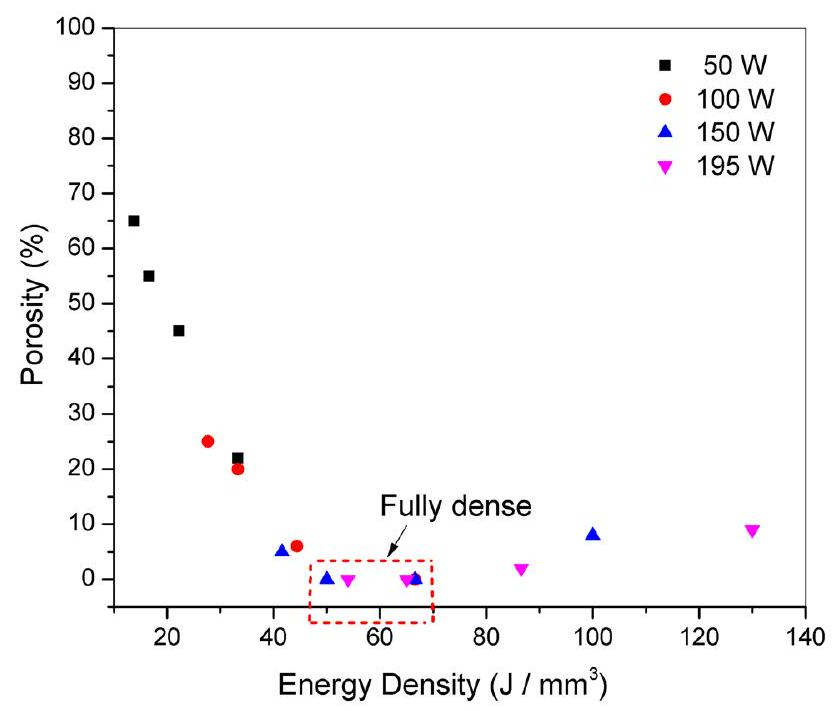
\includegraphics[max width=\textwidth]{2024_02_28_5b6806184856c64a957ag-08}
\end{center}

Fig. 8 Plot showing variation of porosity with respect to energy density\\
As described earlier, in SLM material addition takes place due to layer-by-layer melting and solidification of a thin layer of spread powder. In this process, the laser beam also re-melts some portion of the layers beneath to ensure good bonding between the layers. The solidification of the alloy begins with the formation of a $\beta$ nucleus, and the preexisting $\beta$ grains partially undergo melting and serve as heterogeneous sites for nucleation. Thus, newly formed $\beta$ will grow epitaxially in the build direction or opposite to the heat extraction $[15,23]$. In close similarity to the weld solidification, the solidifying $\beta$ grains tend to orient towards the moving heat source (laser beam), resulting in a slightly tilted grain structure. Further, the $\beta$ grain orientation in the deposit highly depends on the laser power, scanning strategy and scan speed applied. They define the amount of time available for the melt to solidify at any particular instance of time [24]. The solidified high-temperature $\beta$ (bcc) phase is unstable at lower temperatures and will transform (below $M_{\mathrm{s}}$ ) to a metastable phase, martensitic $\alpha^{\prime}$ (hcp) phase by a shear-diffusion less reaction since the cooling rates in SLM are high $\left(10^{8}-10^{5} \mathrm{~K} / \mathrm{s}\right)$ [17]. Hence, the final resultant microstructure will have coarse columnar grains, which are highly oriented towards the build direction with martensite $\alpha^{\prime}$ inside the grains $[10,17,25]$. Due to the inherent layerby-layer deposition method, as a new layer is being deposited a narrow region (heat affected zone) close to the melt pool boundary will reach temperatures above the transformation temperature $\left(990^{\circ} \mathrm{C}\right)$, and martensite $\left(\alpha^{\prime}\right)$ transforms back to the high-temperature $\beta$ phase $[12,17,25]$. As the laser beam traverses away, the high-temperature $\beta$ phase, under faster cooling conditions will transform to martensite $\left(\alpha^{\prime}\right)$. The martensite formed from re-heating of primary martensite $\left(\alpha^{\prime}\right)$ to $\beta$ phase and transformed back to martensite will be from here on referred to as $\alpha^{\prime}{ }_{\text {(secondary) }}$ and the heat affected regions (areas colored in blue Fig. 10) result in $\alpha^{\prime}$ (tertiary). In other words, as the build progresses, the layers will experience multiple thermal cycling effects which lead to the formation of alternate areas of martensite $\alpha^{\prime}$ (primary), $\alpha^{\prime}$ (secondary) and $\alpha_{\text {(tertiary) }}^{\prime}$ in the entire part [17]. A schematic presented in Fig. 9 illustrates the evolution of microstructure in the selective laser melted Ti-6Al-4V alloy. Although it is difficult to draw a clear line between the three martensites $\left(\alpha_{\text {(primary) }}^{\prime}, \alpha_{\text {(secondary) }}^{\prime}\right.$ and $\left.\alpha_{\text {(tertiary) }}^{\prime}\right)$ in the as-built part

\begin{center}
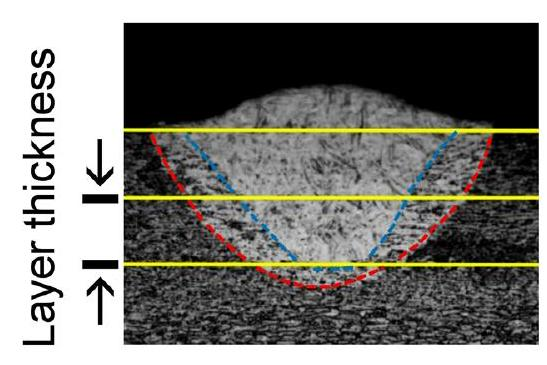
\includegraphics[max width=\textwidth]{2024_02_28_5b6806184856c64a957ag-09}
\end{center}

\section*{Single-track}
\section*{Multi-layer}
\begin{center}
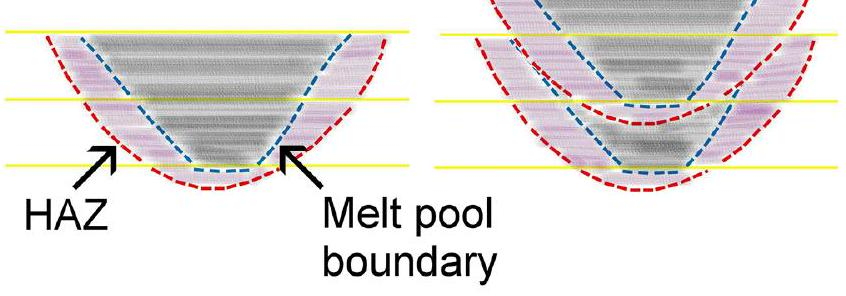
\includegraphics[max width=\textwidth]{2024_02_28_5b6806184856c64a957ag-09(1)}
\end{center}

\section*{Multi -track and multi-layer}
\begin{center}
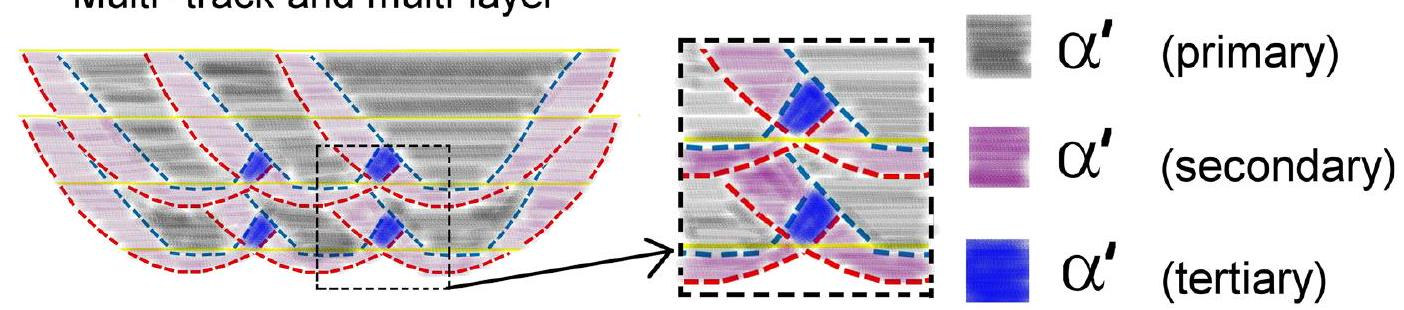
\includegraphics[max width=\textwidth]{2024_02_28_5b6806184856c64a957ag-09(3)}
\end{center}

Fig. 9 A schematic illustration of microstructural evolution in a single-track, multi-layer, and multi-track, multi-layer Ti-6Al-4V SLM deposit

microstructures it is important to understand the microstructural evolution of the alloy during the SLM process. In summary, the part will have preferentially-oriented epitaxial grains with high aspect ratio, with martensite.

A thermal simulation was also carried out for the parameter $195 \mathrm{~W}$ and $1200 \mathrm{~mm} / \mathrm{s}$ to estimate the temperature distribution from the melt pool boundary into the deposit. The temperature distribution plot defines the peak temperatures experienced by the regions while a track of material is being deposited. Therefore, the regions exposed to a temperature above the $\beta$ transus $\left(990{ }^{\circ} \mathrm{C}\right)$ represent the

\begin{center}
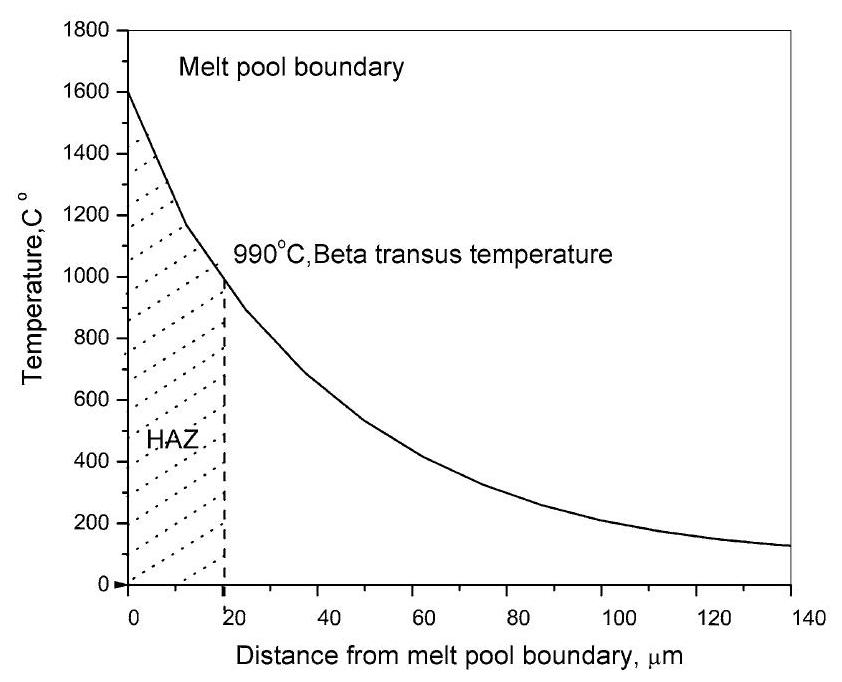
\includegraphics[max width=\textwidth]{2024_02_28_5b6806184856c64a957ag-09(2)}
\end{center}

Fig. 10 Plot from simulated thermal cycle of the melt pool boundary during deposition of a single track of Ti-6Al-4V alloy in SLM extent of heat affected zone converting to $\beta$. The theoretically calculated temperature profiles through simulations closely matched the experimentally observed values (20$25 \mu \mathrm{m}$ ). To obtain the temperature distribution within the heat affected zone, the equation of heat transfer has been used as shown below [26, 27].

$\rho C_{\mathrm{v}} \frac{\partial T}{\partial t}=K\left(\frac{\partial T}{\partial x}+\frac{\partial T}{\partial y}+\frac{\partial T}{\partial z}\right)+Q$

where $\rho$ is the density, $C_{\mathrm{v}}$ is heat capacity, $K$ is the heat conductivity, $T$ is the temperature, and $Q$ is the internal heat generation per unit volume which can be calculated by:

$Q=\int_{v} q \mathrm{~d} v$.

The heat flux $q$ can be approximated by a Gaussian function of laser energy:

$q(x, y)=\frac{2 A P}{\pi \omega^{2}} e^{-\frac{2\left(\omega_{x}^{2}+\omega_{y}^{2}\right)}{\omega^{2}}}$

where $A$ is the absorptivity of laser energy, $P$ is the laser power, $\omega$ is the radius of the laser beam, and $\omega_{x}$ and $\omega_{y}$ are the distance between a point and the center of the laser beam in $x$ and $y$ directions. The temperature ' $T$ ' is solved along each time step of the single bead scan with the consideration of nonlinear temperature dependent Ti-6Al$4 \mathrm{~V}$ thermo-physical properties. The solidus temperature of the alloy Ti-6Al-4V corresponding to the melt pool boundary is taken as $1873 \mathrm{~K}\left(1600{ }^{\circ} \mathrm{C}\right)$ [12, 27]. The melt\\
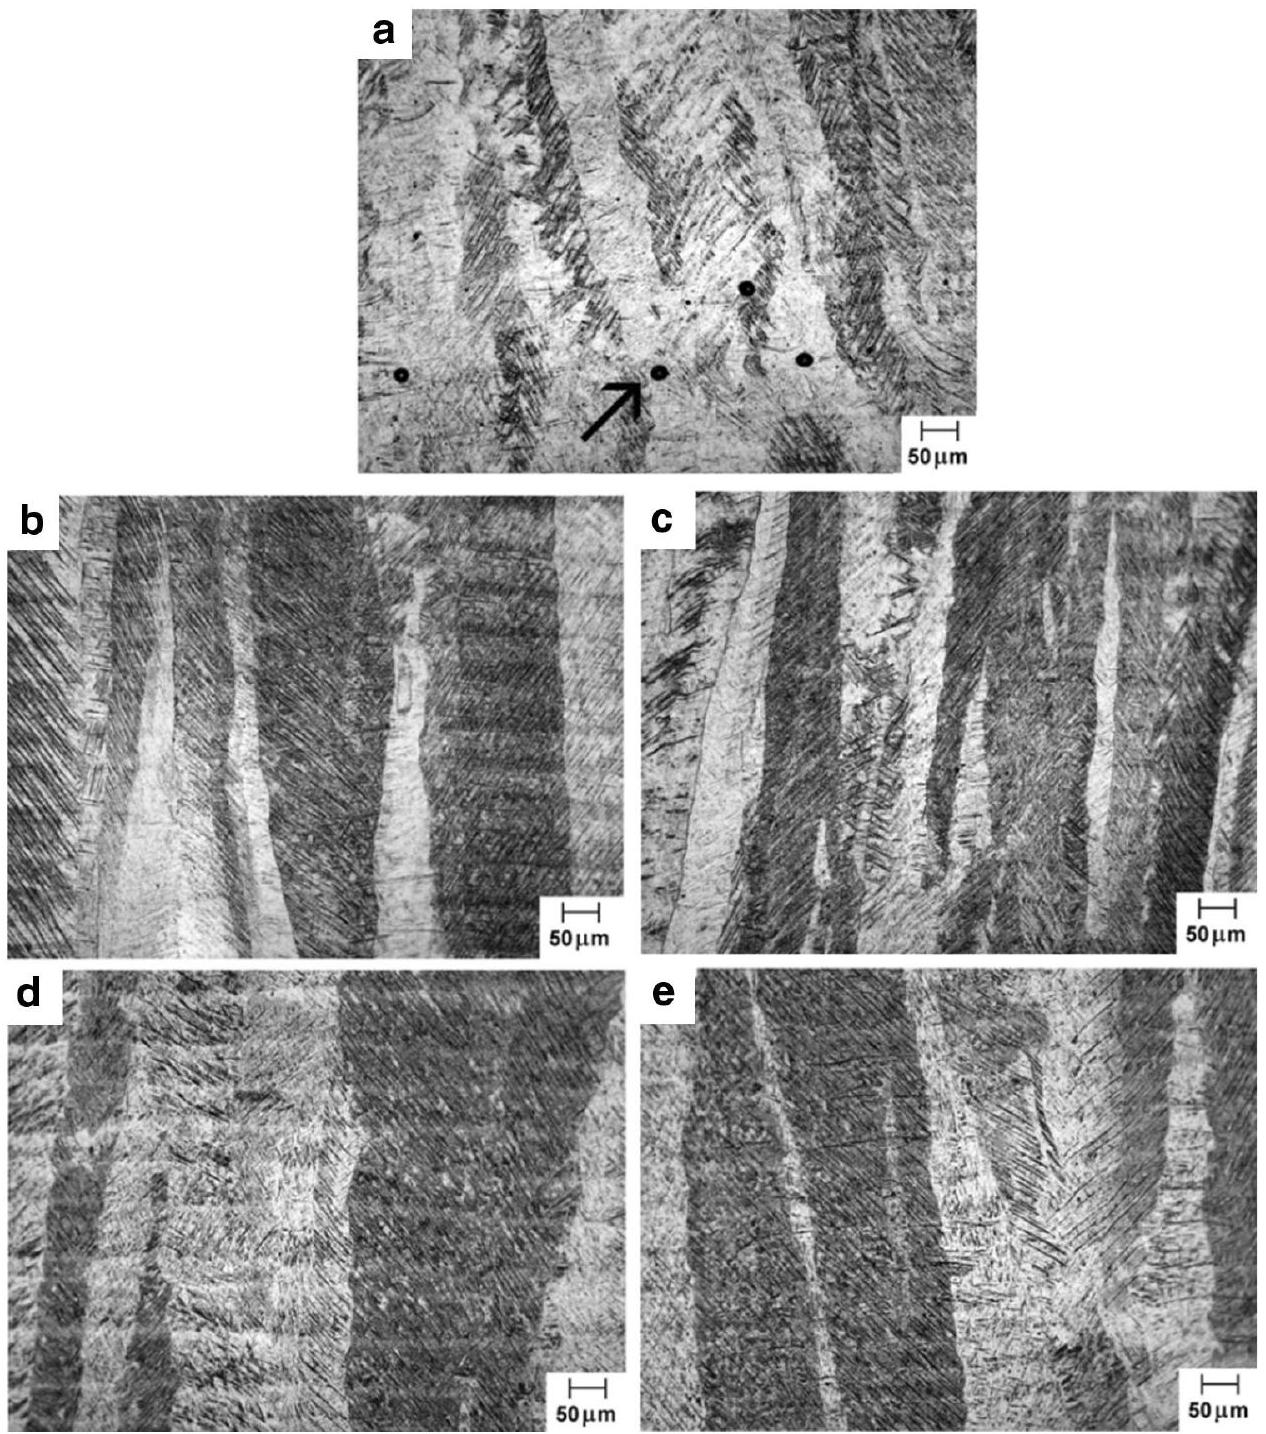
\includegraphics[max width=\textwidth, center]{2024_02_28_5b6806184856c64a957ag-10}

Fig. 11 Typical optical micrographs of a vertical cross-section of the near full dense samples a $100 \mathrm{~W}, 500 \mathrm{~mm} / \mathrm{s}, \mathbf{b} 150 \mathrm{~W}, 750 \mathrm{~mm} / \mathrm{s}, \mathbf{c} 150 \mathrm{~W}$, $1000 \mathrm{~mm} / \mathrm{s}, \mathbf{d} 195 \mathrm{~W}, 1000 \mathrm{~mm} / \mathrm{s}$ and e $195 \mathrm{~W}, 1200 \mathrm{~mm} / \mathrm{s}$

pool shape is obtained by tracking the material state using 3DSIM FLEX simulation software which solves the thermal diffusion problem for a moving laser source step by step. The temperature is recorded and outputted from the center of a melt pool towards the transverse direction with respect to the laser scanning direction. The temperature distribution away from the melt pool is plotted as a function of distance from the melt pool, the plotted region is indicated in Fig. 11.

The optical micrographs of the samples close to full density are presented in Fig. 11. The microstructural features show coarse columnar grains with martensite $\alpha^{\prime}$. The prior $\beta$ grains have their lengths running several millimeters, and the width of the grains was in the range of 80$200 \mu \mathrm{m}$. The cross-section micrograph of the sample built using $100 \mathrm{~W}, 500 \mathrm{~mm} / \mathrm{s}$ showed minor amounts of rounded porosity $(0.4 \%)$. The samples built using 150 and $195 \mathrm{~W}$ produced fully dense parts. The width of the grains was observed to be wider in the case of slower scan speeds, i.e., the samples at the same $150 \mathrm{~W}$ laser power with $750 \mathrm{~mm} / \mathrm{s}$ showed higher grain width when compared to $1000 \mathrm{~mm} / \mathrm{s}$ ones. A similar trend was observed for the samples built using $195 \mathrm{~W}$ with the scan speeds of 1000 and $1200 \mathrm{~mm} / \mathrm{s}$.

\section*{4 Summary}
The present work focuses on the evolution of single-track melt pools and porosity in parts made using SLM of alloy Ti-Al6-4V. The single-track deposits were made using\\
varying laser power and scan speeds, and their effects on the melt pool morphology were studied. Microstructural studies on the melt pool cross-section show that at a low power level and high scan speed the width of the track reduces, gradually becomes discontinuous, and eventually results in balling. The depth of penetration of the melt pool was observed to increase with the lower scan speed. At higher power levels, in some cases a keyhole effect was observed.

The bulk parts produced using parameters similar to single-track deposits showed a direct correlation to the energy density applied and the porosity evolution in the process. Characterization of the cross-sections of the bulk parts demonstrates a good correlation between the singletrack melt pool geometry and porosity in the bulk parts. It was learned from this investigation that the process parameters with low energy density and high energy density both result in porosity in the parts, however, due to different reasons. The melt pool information of single-track deposits could be an aid to select a process window determining an optimum set of process parameters. SLM processing parameters with $150 \mathrm{~W}, 750 \mathrm{~mm} / \mathrm{s}$ and $195 \mathrm{~W}$, $1000 \mathrm{~mm} / \mathrm{s}$ and $1200 \mathrm{~mm} / \mathrm{s}$ result in well-defined bowlshaped melt pools and contribute to near fully dense parts. Therefore, these sets of parameters could be recommended to produce denser parts in the Ti-6Al-4V alloy using selective laser melting.

\section*{References}
\begin{enumerate}
  \item Gibson I, Rosen D, Stucker B (2010) Additive manufacturing technologies: rapid prototyping to direct digital manufacturing. Springer

  \item Rafi HK, Karthik NV, Gong H, Starr TL, Stucker BE (2013) Microstructures and mechanical properties of Ti6Al4V parts fabricated by selective laser melting and electron beam melting. J Mater Eng Perform 22(12):3872-3883

  \item Thompson SM, Bian L, Shamsaei N, Yadollahi A (2015) An overview of direct laser deposition for additive manufacturing; part i: transport phenomena, modeling and diagnostics. Addit Manuf 8:36-62

  \item Baufeld B, Van der Biest O, Dillien S (2010) Texture and crystal orientation in Ti-6Al-4V builds fabricated by shaped metal deposition. Metall Mater Trans A 41(8):1917-1927

  \item Wang F, Williams S, Colegrove P, Antonysamy AA (2013) Microstructure and mechanical properties of wire and arc additive manufactured Ti-6Al-4V. Metall Mater Trans A 44(2):968977

  \item Dilip JJS, Miyanaji H, Lassell A, Starr TL, Stucker B (2017) A novel method to fabricate TiAl intermetallic alloy 3D parts using additive manufacturing. Def Technol 13(2):72-76

  \item Dilip JJS, Janaki Ram GD (2014) Friction freeform fabrication of superalloy Inconel 718: prospects and problems. Metall Mater Trans A 45(1):182-192

  \item Elahinia M et al (2016) Fabrication of NiTi through additive manufacturing: a review. Prog Mater Sci 83:630-663

  \item Collings EW (1984) The physical metallurgy of titanium alloys. American Society for Metals, Technology \& Engineering, Ohio

  \item Al-Bermani SS, Blackmore ML, Zhang W, Todd I (2010) The origin of microstructural diversity, texture, and mechanical properties in electron beam melted Ti-6A1-4V. Metall Mater Trans A 41(13):3422-3434

  \item Anam M, Dilip JJS, Pal D, Stucker B (2016) A short study on the fabrication of single track deposits in SLM and characterization. In: 27th Solid freeform fabrication symposium, Austin, Texas

  \item Gong H, Rafi K, Gu H, Starr T, Stucker B (2014) Analysis of defect generation in Ti-6Al- $\mathrm{V}$ parts made using powder bed fusion additive manufacturing processes. Addit Manuf 1-4:87-98

  \item Gong H, Zeng K, Dilip JJS, Pal D, Stucker B (2014) Melt pool characterization for selective laser melting of Ti-6Al-4V pre-alloyed powder. In: Solid freeform fabrication symposium, University of Texas, Austin, pp 256-267

  \item Xu W, Sun S, Elambasseril J, Liu Q, Brandt M, Qian M (2015) Ti-6Al-4V additively manufactured by selective laser melting with superior mechanical properties. JOM 67(3):668-673

  \item Thijs L, Verhaeghe F, Craeghs T, Humbeeck JV, Kruth J-P (2010) A study of the microstructural evolution during selective laser melting of Ti-6Al-4V. Acta Mater 58(9):3303-3312

  \item Yang J, Han J, Yu H, Yin J, Gao M, Wang Z, Zeng X (2016) Role of molten pool mode on formability, microstructure and mechanical properties of selective laser melted Ti-6Al-4V alloy. Mater Des 110:558-570

  \item Yang J, Yu H, Yin J, Gao M, Wang Z, Zeng X (2016) Formation and control of martensite in Ti-6Al-4V alloy produced by selective laser melting. Mater Des 108:308-318

  \item Yang L, Gong H, Dilip JJS, Stucker B (2014) Solid freeform fabrication symposium, University of Texas, Austin, pp 714-731

  \item Svenungsson J, Choquet I, Kaplan AFH (2015) Laser welding process-a review of Keyhole welding modelling. Phys Proc 78:182-191

  \item Verhaeghe F, Craeghs T, Heulens J, Pandelaers L (2009) A pragmatic model for selective laser melting with evaporation. Acta Mater 57(20):6006-6012

  \item Akman E, Demir A, Canel T, Sinmazçelik T (2009) Laser welding of Ti6Al4V titanium alloys. J Mater Process Technol 209(8):3705-3713

  \item Gao X-L, Zhang L-J, Liu J, Zhang J-X (2014) Porosity and microstructure in pulsed Nd:YAG laser welded Ti6Al4V sheet. J Mater Process Technol 214(7):1316-1325

  \item Kou S (2003) Welding metallurgy. Wiley, New Jersey

  \item Zhao X, Li S, Zhang M, Liu Y, Sercombe TB, Wang S, Hao Y, Yang R, Murr LE (2016) Comparison of the microstructures and mechanical properties of $\mathrm{Ti}-6 \mathrm{Al}-4 \mathrm{~V}$ fabricated by selective laser melting and electron beam melting. Mater Des 95:21-31

  \item Kelly SM, Kampe SL (2004) Microstructural evolution in laserdeposited multilayer Ti-6Al-4V builds: part I. Microstructural characterization. Metall Mater Trans A 35(6):1861-1867

  \item Krieth F, Bohn MS (1986) Principles of heat transfer, 4th edn. Harper and row publishers, New York

  \item Teng C, Gong H, Szabo A, Dilip JJS, Ashby K, Zhang S, Patil N, Pal D, Stucker B (2016) Simulating melt pool shape and lack of fusion porosity for selective laser melting of cobalt chromium components. J Manuf Sci Eng 139(1):011009

\end{enumerate}


\end{document}